\chapter{Data storage and access}

Typically, modern relational databases have shown little efficiency in certain applications using intensive data, like indexing of a large number of documents, sites rendering with high traffic, and streaming sites. Typical RDBMS implementations are tuned either for small but frequent reads and writes or a large set of transactions that have few write accesses. On the other hand NoSQL can serve load lots of reads and writes.\\

We will start making a short overview of the relational model using Postgresql RDMS. Then we move to the NoSQL alternative, through Mongo database.\\

\section{Relational Database Management System}

ToDo

\subsection{Postgresql}

PostgreSQL is a powerful, open source object-relational database system. It has more than 15 years of active development and a proven architecture that has earned it a strong reputation for reliability, data integrity, and correctness. It runs on all major operating systems, including Linux, UNIX (AIX, BSD, HP-UX, SGI IRIX, Mac OS X, Solaris, Tru64), and Windows. It is fully ACID compliant, has full support for foreign keys, joins, views, triggers, and stored procedures (in multiple languages). It includes most SQL:2008 data types, including INTEGER, NUMERIC, BOOLEAN, CHAR, VARCHAR, DATE, INTERVAL, and TIMESTAMP. It also supports storage of binary large objects, including pictures, sounds, or video. It has native programming interfaces for C/C++, Java, .Net, Perl, Python, Ruby, Tcl, ODBC, among others, and exceptional documentation. \\

An enterprise class database, PostgreSQL boasts sophisticated features such as Multi-Version Concurrency Control (MVCC), point in time recovery, tablespaces, asynchronous replication, nested transactions (savepoints), online/hot backups, a sophisticated query planner/optimizer, and write ahead logging for fault tolerance. It supports international character sets, multibyte character encodings, Unicode, and it is locale-aware for sorting, case-sensitivity, and formatting. It is highly scalable both in the sheer quantity of data it can manage and in the number of concurrent users it can accommodate. There are active PostgreSQL systems in production environments that manage in excess of 4 terabytes of data. Some general PostgreSQL limits are included in the table below.\\

PostgreSQL runs stored procedures in more than a dozen programming languages, including Java, Perl, Python, Ruby, Tcl, C/C++, and its own PL/pgSQL, which is similar to Oracle's PL/SQL. Included with its standard function library are hundreds of built-in functions that range from basic math and string operations to cryptography and Oracle compatibility. Triggers and stored procedures can be written in C and loaded into the database as a library, allowing great flexibility in extending its capabilities. Similarly, PostgreSQL includes a framework that allows developers to define and create their own custom data types along with supporting functions and operators that define their behavior. As a result, a host of advanced data types have been created that range from geometric and spatial primitives to network addresses to even ISBN/ISSN (International Standard Book Number/International Standard Serial Number) data types, all of which can be optionally added to the system.\\

Just as there are many procedure languages supported by PostgreSQL, there are also many library interfaces as well, allowing various languages both compiled and interpreted to interface with PostgreSQL. There are interfaces for Java (JDBC), ODBC, Perl, Python, Ruby, C, C++, PHP, Lisp, Scheme, and Qt just to name a few.\\

Best of all, PostgreSQL's source code is available under a liberal open source license: the PostgreSQL License. This license gives you the freedom to use, modify and distribute PostgreSQL in any form you like, open or closed source. Any modifications, enhancements, or changes you make are yours to do with as you please. As such, PostgreSQL is not only a powerful database system capable of running the enterprise, it is a development platform upon which to develop in-house, web, or commercial software products that require a capable RDBMS.\\


\begin{center}
\begin{tabular}{|l|l|}
\hline \textbf{Limit} & \textbf{Value}\\ \hline
Maximum Database Size & Unlimited\\
Maximum Table Size & 32 TB\\
Maximum Row Size & 1.6 TB\\
Maximum Field Size & 1 GB\\
Maximum Rows per Table & Unlimited\\
Maximum Columns per Table & 250 - 1600 depending on column types\\
Maximum Indexes per Table & Unlimited\\ \hline
\end{tabular}
\end{center}


\begin{figure}
\centering
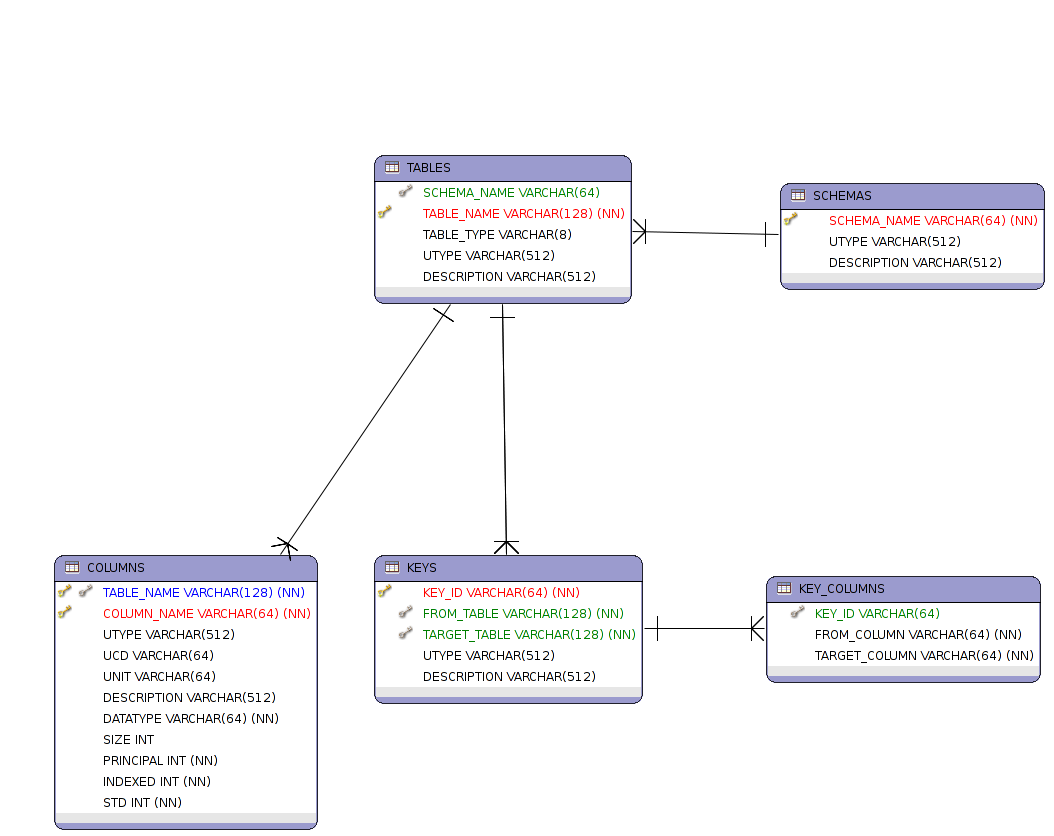
\includegraphics[width=11cm,height=8cm]{images/erd_postgres.png}\\
\caption{Entity-Relationship Diagram for VO Tap Schema}
\end{figure}


\section{NoSQL}

NoSQL implementations used in the real world include 3TB Digg green markers (indicated to highlight the stories voted by others in the social network), the 6 TB of "ENSEMBLE" European Commission database used in comparing models and air quality, and the 50 TB of Facebook inbox search.\\

NoSQL architectures often provide limited consistency, such as events or transactional consistency restricted to only data items. Some systems, however, provide all guarantees offered by ACID systems by adding an intermediate layer. There are two systems that have been deployed and provide for storage of snapshot isolation column: Google Percolator (based on BigTable system) and Hbase transactional system developed by the University of Waterloo. These systems use similar concepts in order to achieve distributed multiple rows ACID transactions with snapshot isolation guarantees for the underlying storage system in that column, wit no extra overhead in data management, no system deployment middleware or any maintenance introduced by middleware layer.\\

Quite NoSQL systems employ a distributed architecture, maintaining data redundantly on multiple servers, often using distributed hash table. Thus, the system may actually escale adding more servers, and thus a server failure may be tolerated.\\

There are different NoSQL DBs for different projects:

\begin{itemize}

\item Document oriented

  \begin{itemize}
    \item CouchDB
    \item MongoDB
    \item RavenDB
    \item BaseX
    \item djondb
    \item eXist
    \item SimpleDB
    \item IBM Lotus Domino
    \item Terrastore
  \end{itemize}

\item Graph oriented

  \begin{itemize}
    \item Neo4j
    \item DEX
    \item AllegroGraph
    \item OrientDB
    \item InfiniteGraph
    \item Sones GraphDB
    \item InfoGrid
    \item HyperGraphDB
  \end{itemize}

\item Key-value oriented

  \begin{itemize}
    \item Cassandra
    \item BigTable
    \item Dynamo (Amazon)
    \item MongoDB
    \item Project Voldemort (LinkedIn)
    \item Riak
    \item Redis
  \end{itemize}

\item Multivalue

  \begin{itemize}
    \item OpenQM
    \item Extensible storage engine
  \end{itemize}  

\item Object Oriented
  
  \begin{itemize}
    \item Zope Object Database
    \item db4o
    \item GemStone S
    \item Objectivity/DB
  \end{itemize}

\item Tabular

  \begin{itemize}
    \item HBase
    \item BigTable
    \item LevelDB (BigTable open version)
    \item Hypertable
  \end{itemize}
  

\end{itemize}

They run on clusters of inexpensive machines.\\



\subsection{MongoDB}

MongoDB (from "humongous") is an open source document-oriented database system developed and supported by 10gen. It is part of the NoSQL family of database systems. Instead of storing data in tables as is done in a "classical" relational database, MongoDB stores structured data as JSON-like documents with dynamic schemas (MongoDB calls the format BSON), making the integration of data in certain types of applications easier and faster. \\

10gen began Development of MongoDB in October 2007 and was not created to be just another database that tries to do everything for everyone. Instead, MongoDB was created to work with documents rather than rows, was extremely fast, massively scalable, and easy to use. In order to accomplish this, some features were excluded, namely support for transactions.

\subsubsection{Main features}

\begin{itemize}

\item Ad hoc queries
MongoDB supports search by field, range queries, regular expression searches. Queries can return specific fields of documents and also include user-defined JavaScript functions.

\item Indexing
Any field in a MongoDB document can be indexed (indices in MongoDB are conceptually similar to those in RDBMSes). Secondary indices are also available.

\item Replication
MongoDB supports master-slave replication. A master can perform reads and writes. A slave copies data from the master and can only be used for reads or backup (not writes). The slaves have the ability to select a new master if the current one goes down.

\item Load balancing
MongoDB scales horizontally using sharding.[9] The developer chooses a shard key, which determines how the data in a collection will be distributed. The data is split into ranges (based on the shard key) and distributed across multiple shards. (A shard is a master with one or more slaves.)
MongoDB can run over multiple servers, balancing the load and/or duplicating data to keep the system up and running in case of hardware failure. Automatic configuration is easy to deploy and new machines can be added to a running database.

\item File storage
MongoDB could be used as a file system, taking advantage of load balancing and data replication features over multiple machines for storing files.
This function, called GridFS,[10] is included with MongoDB drivers and available with no difficulty for development languages (see "Language Support" for a list of supported languages). MongoDB exposes functions for file manipulation and content to developers. GridFS is used, for example, in plugins for NGINX.[11] and lighttpd[12]
In a multi-machine MongoDB system, files can be distributed and copied multiple times between machines transparently, thus effectively creating a load balanced and fault tolerant system.

\item Aggregation
MapReduce can be used for batch processing of data and aggregation operations. The aggregation framework enables users to obtain the kind of results for which the SQL GROUP BY clause is used.

\item Server-side JavaScript execution
JavaScript can be used in queries, aggregation functions (such as MapReduce), are sent directly to the database to be executed.

\item Capped collections
MongoDB supports fixed-size collections called capped collections. This type of collection maintains insertion order and, once the specified size has been reached, behaves like a circular queue.

Once we have seen the main features of MongoDB, we can move on to the language itself.
\end{itemize}


\subsubsection{The basics}

We must know four concepts to dig into MongoDB's world:

\begin{itemize}
\item Database: this concept is much like the RDBM counterpart.
\item Collection: we can see a collection and a table as the same thing.
\item Document: its equivalent in RDBM is the row, and a document is made up of fields.
\item Field: is a lot like a column.
\end{itemize}


\begin{figure}
\centering
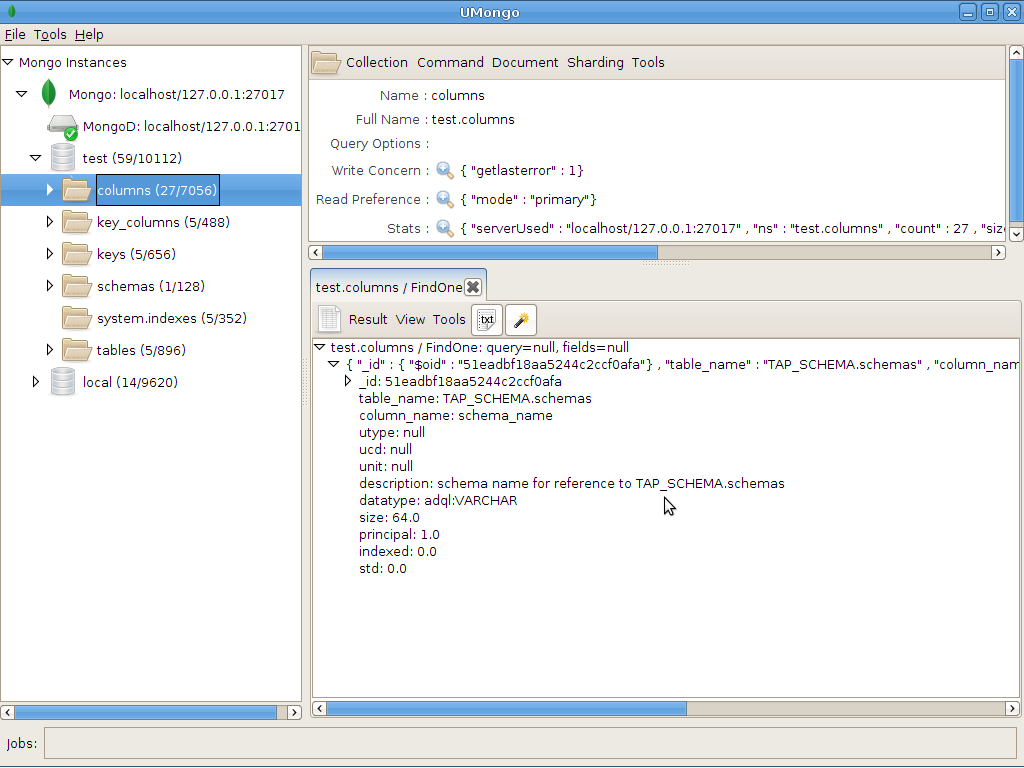
\includegraphics[width=11cm,height=8cm]{images/mongo_dia.png}\\
\caption{Tree View for Tap Schema in MongoVue}
\end{figure}


\subsection{Advantages and uncertainties of using a NoSQL solution}

\begin{itemize}

\item Elastic scaling

For years, database administrators have relied on scale up — buying bigger servers as database load increases — rather than scale out — distributing the database across multiple hosts as load increases. However, as transaction rates and availability requirements increase, and as databases move into the cloud or onto virtualized environments, the economic advantages of scaling out on commodity hardware become irresistible.

RDBMS might not scale out easily on commodity clusters, but the new breed of NoSQL databases are designed to expand transparently to take advantage of new nodes, and they’re usually designed with low-cost commodity hardware in mind.


\item Big data

Just as transaction rates have grown out of recognition over the last decade, the volumes of data that are being stored also have increased massively. O’Reilly has cleverly called this the “industrial revolution of data.” RDBMS capacity has been growing to match these increases, but as with transaction rates, the constraints of data volumes that can be practically managed by a single RDBMS are becoming intolerable for some enterprises. Today, the volumes of “big data” that can be handled by NoSQL systems, such as Hadoop, outstrip what can be handled by the biggest RDBMS.


\item No need for DBAs

Despite the many manageability improvements claimed by RDBMS vendors over the years, high-end RDBMS systems can be maintained only with the assistance of expensive, highly trained DBAs. DBAs are intimately involved in the design, installation, and ongoing tuning of high-end RDBMS systems.

NoSQL databases are generally designed from the ground up to require less management:  automatic repair, data distribution, and simpler data models lead to lower administration and tuning requirements — in theory. In practice, it’s likely that rumors of the DBA’s death have been slightly exaggerated. Someone will always be accountable for the performance and availability of any mission-critical data store.


\item Economics

NoSQL databases typically use clusters of cheap commodity servers to manage the exploding data, while RDBMS tends to rely on expensive proprietary servers and storage systems. The result is that the cost per gigabyte or transaction/second for NoSQL can be many times less than the cost for RDBMS, allowing you to store and process more data at a much lower price point.


\item Flexible data models

Change management is a big headache for large production RDBMS. Even minor changes to the data model of an RDBMS have to be carefully managed and may necessitate downtime or reduced service levels.

NoSQL databases have far more relaxed — or even nonexistent — data model restrictions. NoSQL Key Value stores and document databases allow the application to store virtually any structure it wants in a data element. Even the more rigidly defined BigTable-based NoSQL databases (Cassandra, HBase) typically allow new columns to be created without too much fuss.

The result is that application changes and database schema changes do not have to be managed as one complicated change unit. In theory, this will allow applications to iterate faster, though,clearly, there can be undesirable side effects if the application fails to manage data integrity.

\end{itemize}


NoSQL systems have generated a lot of enthusiasm but there are still a lot of questions about its future:

\begin{itemize}

\item Maturity

RDBMS systems have been around for a long time. NoSQL advocates will argue that their advancing age is a sign of their obsolescence, but for most CIOs, the maturity of the RDBMS is reassuring. For the most part, RDBMS systems are stable and richly functional. In comparison, most NoSQL alternatives are in pre-production versions with many key features yet to be implemented.

Living on the technological leading edge is an exciting prospect for many developers, but enterprises should approach it with extreme caution.

\item Support

Enterprises want the reassurance that if a key system fails, they will be able to get timely and competent support. All RDBMS vendors go to great lengths to provide a high level of enterprise support.

In contrast, most NoSQL systems are open source projects, and although there are usually one or more firms offering support for each NoSQL database, these companies often are small start-ups without the global reach, support resources, or credibility of an Oracle, Microsoft, or IBM.

\item Analytics and business intelligence

NoSQL databases have evolved to meet the scaling demands of modern Web 2.0 applications. Consequently, most of their feature set is oriented toward the demands of these applications. However, data in an application has value to the business that goes beyond the insert-read-update-delete cycle of a typical Web application. Businesses mine information in corporate databases to improve their efficiency and competitiveness, and business intelligence (BI) is a key IT issue for all medium to large companies.

NoSQL databases offer few facilities for ad-hoc query and analysis. Even a simple query requires significant programming expertise, and commonly used BI tools do not provide connectivity to NoSQL.

Some relief is provided by the emergence of solutions such as HIVE or PIG, which can provide easier access to data held in Hadoop clusters and perhaps eventually, other NoSQL databases. Quest Software has developed a product — Toad for Cloud Databases — that can provide ad-hoc query capabilities to a variety of NoSQL databases.

\item Administration

The design goals for NoSQL may be to provide a zero-admin solution, but the current reality falls well short of that goal. NoSQL today requires a lot of skill to install and a lot of effort to maintain.

\item Expertise

There are literally millions of developers throughout the world, and in every business segment, who are familiar with RDBMS concepts and programming. In contrast, almost every NoSQL developer is in a learning mode. This situation will address naturally over time, but for now, it is by far easier to find experienced RDBMS programmers or administrators than NoSQL experts.

\end{itemize}

%\section{Languages}

%\subsection{Java}

%Java is a general-purpose, concurrent, class-based, object-oriented computer programming language that is specifically designed to have as few implementation dependencies as possible. It is intended to let application developers "write once, run anywhere", meaning that code that runs on one platform does not need to be recompiled to run on another. Java applications are typically compiled to bytecode (class file) that can run on any Java virtual machine (JVM) regardless of computer architecture.

%We have selected the Java for our study because of its availability and the huge amount of tools ready to use for software development. Its also really easy to set up a development environment, just in a couple of click we can have our IDE configured to start working. See the appendices for more information on how to get a fully operating set of tools.